\chapter{Evaluierung von Open API 2.0 Plug-In von OWASP ZAP}
\label{cha:k5}

Die in Abschnitt \ref{ablaufpentest} vorgestellten Schritte eines Penetrationstests werden in diesem Kapitel zur Evaluierung von Open API 2.0 Plug-In von OWASP ZAP herangezogen. Um die bereits entwickelte Springboot Anwendung nach Sicherheitslücken zu testen, werden mit Hilfe des Open API 2.0 Plug-Ins von OWASP ZAP die Penetrationstests durchgeführt.

\section{Ablauf des Open API 2.0 Plug-In von OWASP ZAP}

\subsection{Vorbereitung}

In der Vorbereitungsphase werden die entsprechende Anforderungen für einen Penetrationstest erfüllt, um eine sichere Anwendung zu entwickeln. Hier wird bestimmt, welche Komponente dem Test unterzogen werden. Mittels Springboot kann automatisiert eine Dokumentation der REST API als Swagger 2.0 generiert werden. Die automatisch generierten Restdoc werden in das OpenAPI 2.0 Plug-In von OWASP-ZAP importiert und die geeigneten REST-API-Sicherheitstests für die Schwachstellen durchgeführt. Außerdem kann dieser Penetrationstest in das Konzept des White-Box-Tests eingestuft werden, da vollständige Kenntnisse der zu testenden Infrastruktur vorliegt.

\subsection{Informationsbeschaffung}

Nun, da die Vorbereitungsphase abgeschlossen ist, ist es soweit, mit der Beschaffung von Information über die Springboot Anwendung anzufangen. Diese Springboot Anwendung (Online Shop) enthält bestimmte Produkte. Durch die REST API können Produkte aufgerufen, angezeigt, hinzugefügt, aktualisiert und gelöscht werden. Normalerweiße wird ein Portscan gegen das Zielsystem durchgeführt, um einen Überblick zu bekommen welche Dienste erreichbar sind, aber in dem Fall brauchen wir Portscan nicht, weil automatisch durch das OpenAPI 2.0 Plug-In alle erreichbare Dienste aufgerufen werden können.  Zusätzlich ist zu erwähnen, dass bereits bekannt ist, welche Funktionalitäten diese Springboot-Anwendung besitzt, weshalb in dieser Phase nicht viel Zeit zu investieren ist.

\subsection{Bewertung der Informationen und Risikoanalyse}

In der vorherigen Phase werden alle notwendigen Informationen gesammelt und wird in dieser Phase ausführlich zusammengetragen.
Da ich die Springboot-Anwendung selbst entwickelt habe, wird OWASP-ZAP im  "`Attack Mode"' Penetrationstests durchgeführt und wird auf kein rechtliches Problem gestoßen. Attack Mode bedeutet, dass noch mehr unnötige Informationen in das Programm geladen werden, deshalb ist es wahrscheinlicher das Programm beschädigt und könnte danach vielleicht alle Funktionalitäten nicht erfüllen.

\subsection{Aktive Eindringversuche}

Laut der Risikoanalyse in der dritten Phase können die Penetrationstests für die REST API durchgeführt werden. Durch das OpenAPI 2.0 Plug-In von OWASP ZAP wird in die Springbootanwendung so weit wie möglich vorgedrungen. Da durch den Versuch einzudringen die Springboot-Anwendung beschädigt werden könnten, wird nun eine Schattensystem (eine exakte Kopie des zu testenden Systems) verwendet.\\

\newpage

\begin{figure}[h]
	\centering
	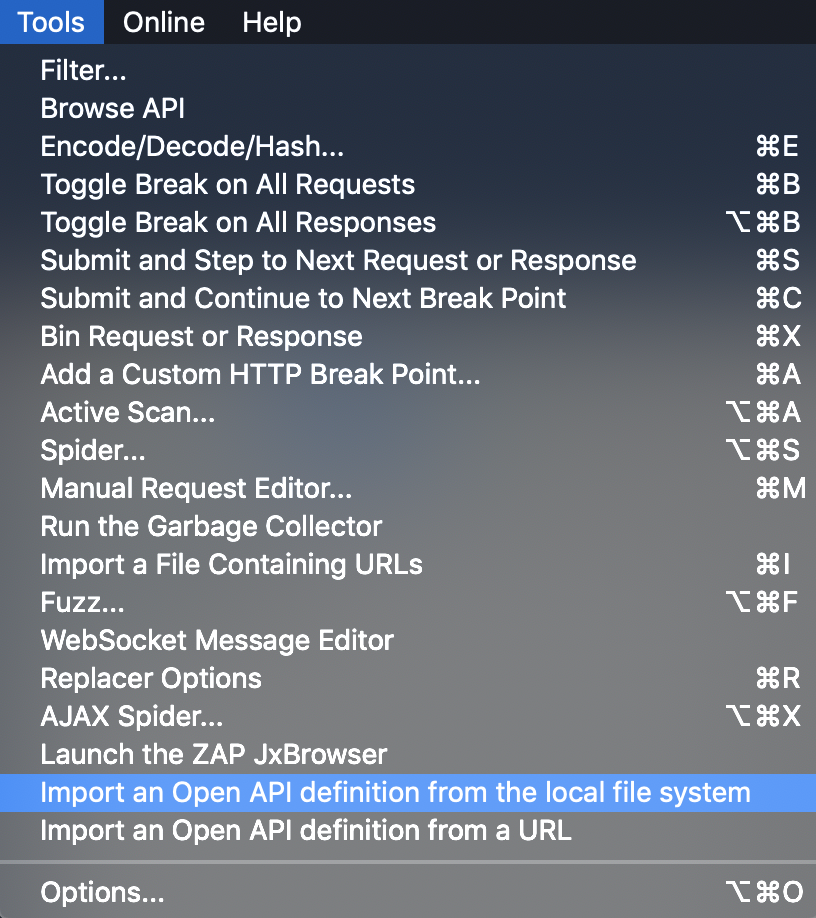
\includegraphics[width=8cm]{2-importbuttonoa2.png}
	\caption{Menuleiste von Open API Plug-In}
	\label{swaggerimport1}
\end{figure}

Um den REST API Penetrationstest durchzuführen, wird von der Menuleiste "`Tools"' geklickt und danach wird "`Import an Open API definition from the local file system"' wie bei der Abbildung \ref{swaggerimport1} gewählt.

\begin{figure}[h]
	\centering
	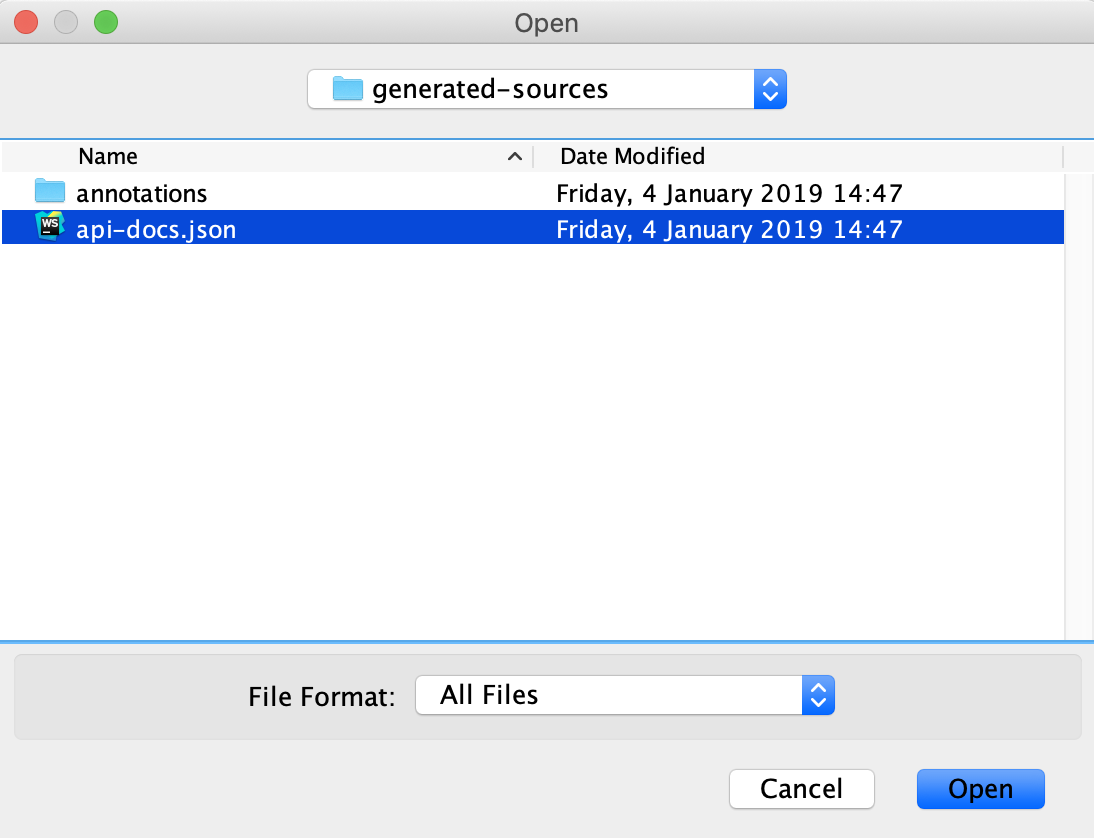
\includegraphics[width=8cm]{3-swaggerfilefortest.png}
	\caption{Importieren von Swagger 2.0 Datei}
	\label{swaggerimport2}
\end{figure}


Wie bei der Abbildung \ref{swaggerimport2} zu sehen, wird lokale Swagger 2.0 Datei ins OWASP ZAP durch das OpenAPI 2.0 Plug-In importiert.

\begin{figure}[h]
	\centering
	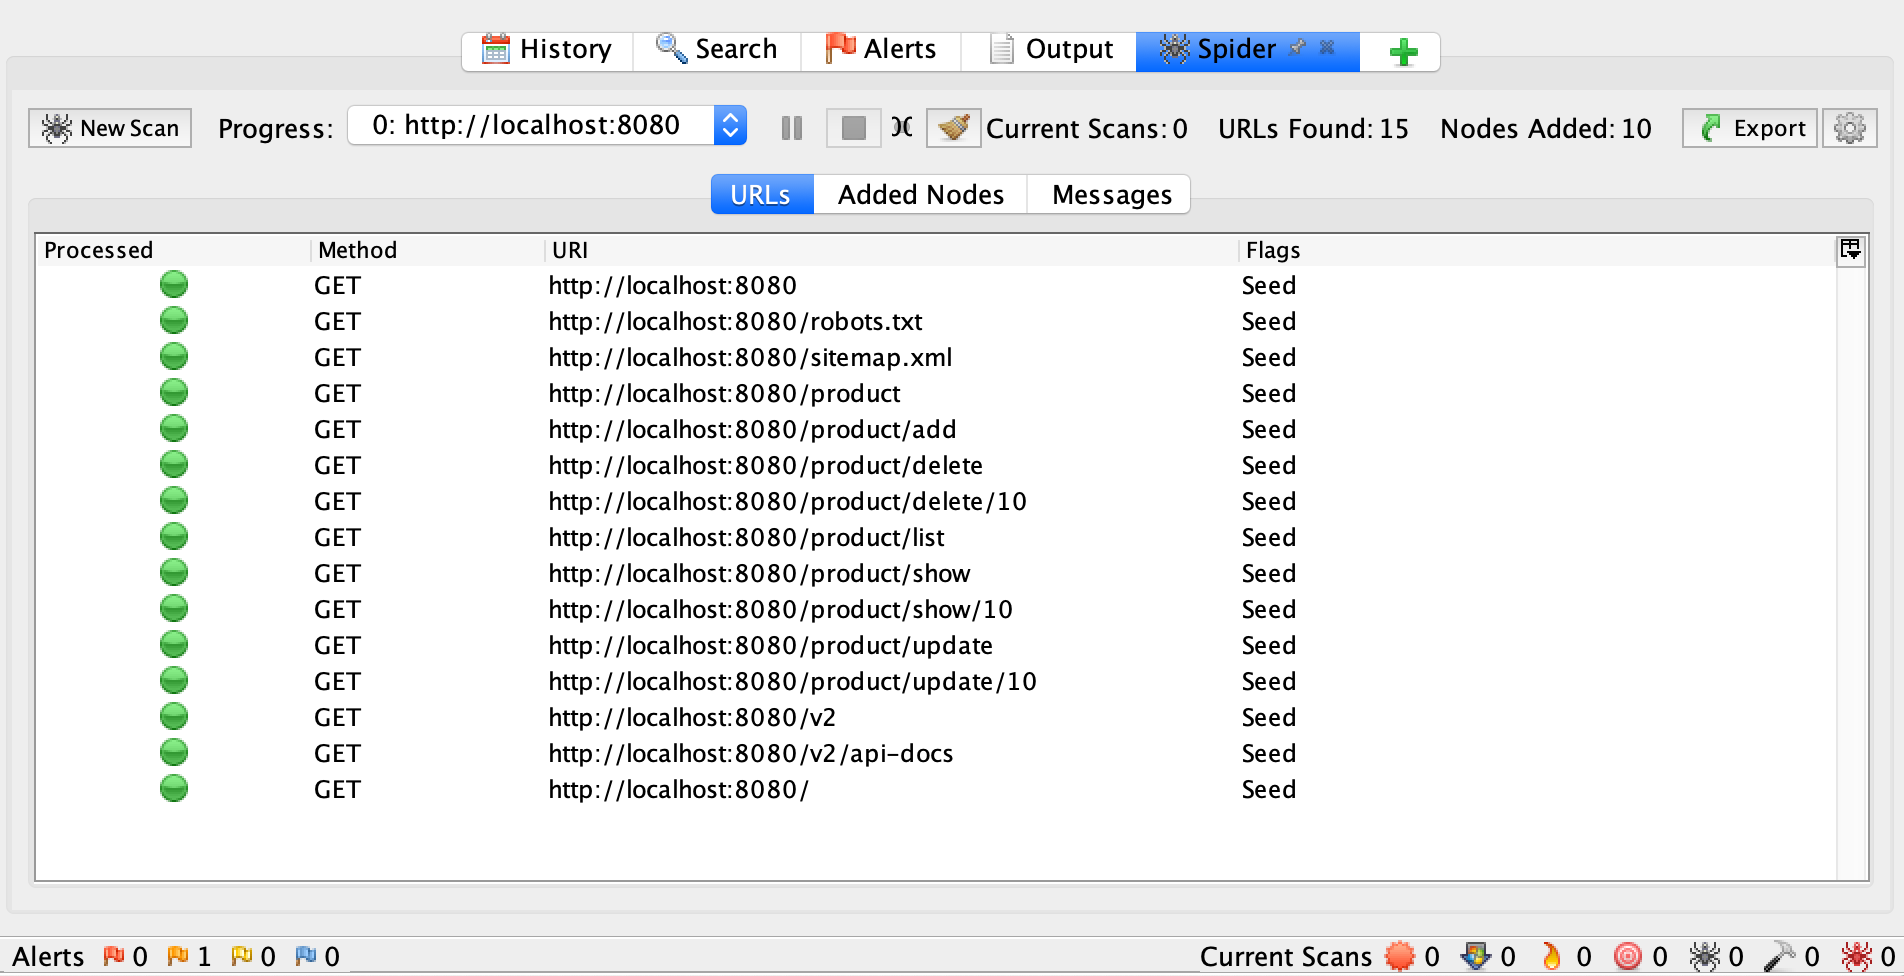
\includegraphics[width=14cm]{5-spiderofurls}
	\caption{Auflistung von erreichbare Diensten}
	\label{swaggerimport3}
\end{figure}

Danach wird durch das Spider alle mögliche Links aufgelistet (siehe \ref{swaggerimport3}), wenn die erreichbar sind. Nun kann mit dem "`Aktive Scan"' wie bei der Abbildung \ref{swaggerimport4} gestartet werden. 

\begin{figure}[h]
	\centering
	\includegraphics[width=14cm]{6-activescancall.png}
	\caption{Aufrufen von Active Scan}
	\label{swaggerimport4}
\end{figure}

Während dem Active Scan-Fortschritt wird unser lokal laufende Springboot-Anwendung für die Sicherheitslücken wie z.B. SQL Injektion, Buffer Overflow, XSS usw. gesucht.

\newpage

Wenn die Suche nach Sicherheitslücken erfolgreich beendet wird, wird alle gefundene Sicherheitslücken wie bei der Abbildung \ref{swaggerimport5} angezeigt.

\begin{figure}[h]
	\centering
	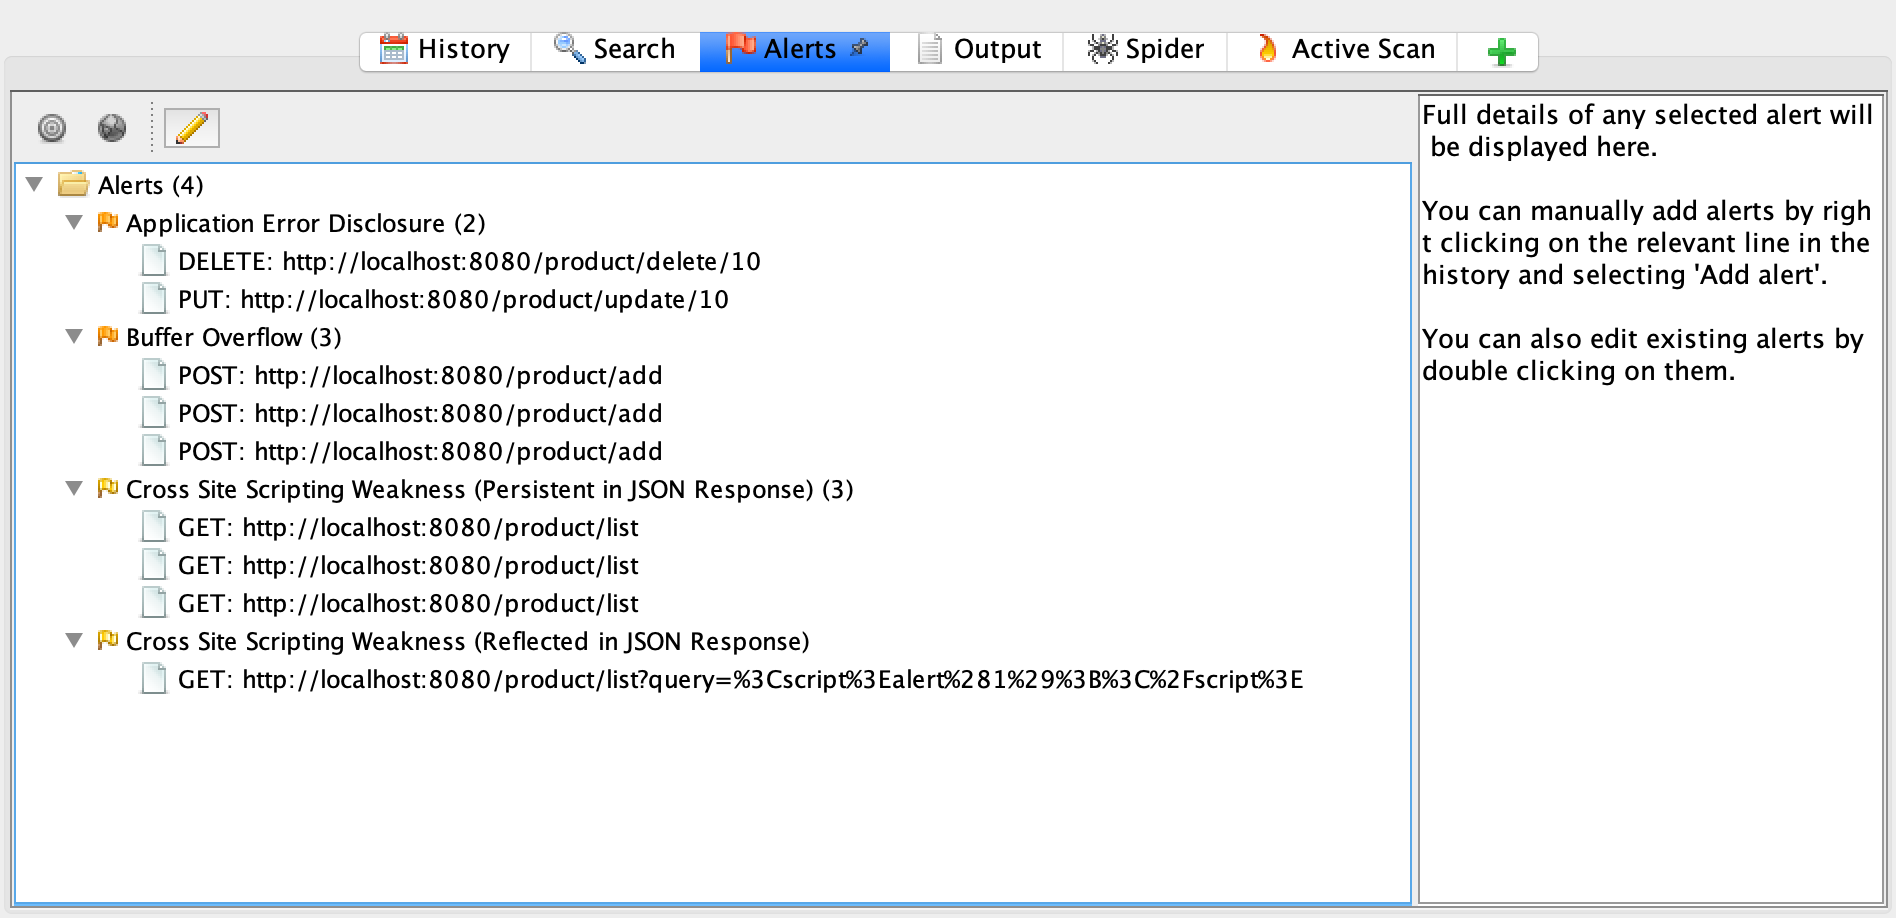
\includegraphics[width=12cm]{7-scanergebnis.png}
	\caption{Ergebnis von Active Scan}
	\label{swaggerimport5}
\end{figure}

\subsection{Abschlussanalyse}

Nach dem Ergebnis des OWASP ZAPs wurden die folgende Sicherheitslücken gefunden;

\begin{itemize}
	\item Application Error Disclosure (2 Stück)
	\item Buffer Overflow (3 Stück)
	\item Cross Site Scripting Weakness (Persistent in JSON Response) (3 Stück)
	\item Cross Site Scripting Weakness (Reflected in JSON Responses)
\end{itemize}

\subsubsection{Vermeidung von Application Error Disclosure}

Wenn eine Anwendung einem Benutzer einen Fehler anzeigt, sollte eine Fehlernachricht die Ursache des Fehlers erklären können. Durch ein normalen Stacktrace kann ein Angreifer zusätzliche Informationen über das System erfahren. 

Zum Beispiel: Wenn ein Benutzer aus Versehen (oder absichtlich) einen \& in einer Inputfeld eingibt, muss die Anwendung anstelle der vollständigen Fehlerdetails einschließlich der Programmierlogik die Meldung "`Fehler aufgrund nicht unterstützter Zeichen. Überprüfen Sie Ihre Eingabe"' anzeigen\cite{ase17}.

\subsubsection{Vermeidung von Buffer Overflow}

Webanwendungen oder Webdienste verwenden Eingaben aus HTTP-Anforderungen (und gelegentlich Dateien), um zu bestimmen, wie sie reagieren sollen. Angreifer können jeden Teil einer HTTP-Anfrage manipulieren, einschließlich der URL, der Abfragezeichenfolge, der Header, der Cookies, der Formularfelder und der ausgeblendeten Felder, um die Sicherheitsmechanismen der Seite zu beschädigen. Der verbreitete Angriff für einen Manipulationsangriff ist der Pufferüberlauf.

Der Server sollte niemals annehmen, dass der Content-Type immer den Inhaltstyp-Header und den Inhalt vom selben Typ überprüft. Ein Mangel an Content-Type-Headern oder unerwarteten Content-Type-Headern sollte dazu führen, dass der Server den Inhalt mit einer \texttt{406 Not Acceptable-Antwort} ablehnt\cite{bofangpre16}.

\subsubsection{Vermeidung von Cross Site Scripting (Persistent)}

Um Persistent XSS am besten zu verhindern, muss sichergestellt werden, dass alle Benutzereingaben ordnungsgemäß bereinigt werden, bevor sie dauerhaft auf dem Webserver gespeichert werden. Außerdem muss die statischen Inhalte, die den Benutzern angezeigt werden, ebenfalls bereinigt werden\cite{xsspersistent14}.

\subsubsection{Vermeidung von Cross Site Scripting (Reflected)}

Web Application Firewalls (WAF) spielen eine wichtige Rolle bei der Abwehr reflektierter XSS-Angriffe. Mit signaturbasierten Sicherheitsregeln kann eine WAF das Fehlen von Eingabebereinigungen ausgleichen und abnormale Anforderungen einfach blockieren. Dies umfasst Anforderungen, die versuchen, einen reflektierten Cross-Site-Scripting-Angriff auszuführen\cite{xssreflected16}.

\newpage

\section{Die Wichtigkeit von automatisierte API Penetrationstesting}

\begin{quote}
	\emph{\\
		"`Design all API security with public access in mind"'}
	\begin{flushright}
		Phillipp Schöne, Axway
	\end{flushright}
\end{quote}

Der Hauptgrund ist, dass die API-Angriffsflächen größer sind. Webanwendungen werden in \texttt{micro-services} aufgeteilt, wodurch eine große Anzahl von Schnittstellen entsteht und diese Schnittstellen dem öffentlichen Internet zugänglich gemacht werden. Dadurch werden zahlreiche Angriffsflächen erstellt, sodass Hacker nicht mehr eine einzelne Anwendung angreifen müssen. Sie können sich eine Vielzahl von Diensten ansehen, wodurch das Risiko erhöht wird, dass sie auf Daten zugreifen können\cite{mswv17}. 

Im Vergleich zu anderen Komponenten ist die API in einer Anwendung die schwächste Verbindung, die ein Hacker nach Datenverletzungen suchen kann. API-Sicherheitstests stellen sicher, dass die API vor Schwachstellen geschützt ist. Der API-Hack einer Anwendung kann Verwirrung auf Organisationsebene verursachen und zu erheblichen Verlusten für die Organisation führen\cite{whyvriticalapi17}. Des Weiteren besteht das größte Problem bei der API- und Microservices-Sicherheit derzeit darin, dass sie häufig als nachträglicher Vorgang betrachtet wird und nicht als wesentlicher Bestandteil des Entwicklungsprozesses\cite{anthonyart18}.

Wenn mit dem Entwickeln der API-Sicherheitstests bis nach der Entwicklung gewartet wird, werden sie natürlich so vorbeireitet, dass nur die günstige Testfälle durchgeführt werden. Sobald eine API oder ein Teil der Software erstellt wurde, wird sich darauf konzentriert, wie sie funktioniert werden soll, aber nicht die anderen wahrscheinlichen Szenarien. Dagegen werden die Penetrationstests durch OpenAPI Plug-In von OWASP ZAP während der Entwicklung durchgeführt und mit Hilfe dieser Situation werden API-Tests nur stärker und umfassender geworden, was dem Team langfristig zugute kommt, die API-Qualität erhöht und die Anzahl der aufgetretenen Fehler verringert. Die Erfassung aller Grundlagen potenzieller Softwarefehler ist eine entscheidende Komponente für die Aufrechterhaltung des Qualitäts- und Kundenvertrauens. Automatisierte API-Tests während der Entwicklung können Probleme mit der API, dem Server, anderen Diensten oder dem Netzwerk aufdecken, die nach der Bereitstellung möglicherweise nicht leicht gefunden oder gelöst werden können. Sobald die Software in der Produktion ist, werden durch OWASP ZAP manuelle Tests erstellt, um neuen und weiterentwickelten Anwendungsfällen zu testen. Restful API-Tests können auf verschiedene Arten in Ihren Entwicklungsprozess integriert werden. Viele Unternehmen bieten API-Tests in ihren Continuous Integration (CI) und Continuous Deployment (CD) Prozessen an. Wenn ein API-Test während CI oder CD fehlschlägt, wird der Prozess angehalten und das API-Problem muss behoben werden, bevor der Build abgeschlossen ist. Die Benutzung des OpenAPI Plug-Ins von OWASP ZAP für automatisierte API-Tests in diesen Prozess gibt den Entwickler mehr Sicherheit, dass alle Grundlagen vor der Veröffentlichung des Produkts für die Kunden abgedeckt wurden\cite{restcaseapiimportance16}.
